\section*{Introduction}

GenBrush is a C library providing structures and functions for creating 2D/3D, bitmap/vector, still/animated graphics on various supports.\\

It can be use as a monolithic library, or as an interface with another graphical library (Cairo/GTK). The choice can be made through a single compilation option.\\

GenBrush is based on the following model: the scene to be represented graphically is composed of Objects viewed by an Eye, interpreted by a Hand and recreated with a Tool applying an Ink on a Surface made of Layers.\\

The currently available implementations for these entities are:\\
\begin{itemize}
\item Object: Point (VecFloat), SCurve, Shapoid
\item Eye: Orthographic, Isometric
\item Hand: Default
\item Tool: PixelPlotter, Pen
\item Ink: Solid
\item Surface: Image (TGA), GBApp, GBWidget
\item Layer: divided into background, inside and foreground layers; blending modes: Default (overwritting), Normal, Over
\end{itemize}
For details refer to the following sections.\\

The library can easily be extended to match the user needs. Foreseen extensions of the entities are for example:\\
\begin{itemize}
\item Object: BBody, ...
\item Eye: Perspective, ...
\item Hand: Human (approximation of the viewed object), ...
\item Tool: Brush, ...
\item Ink: Generic (BBody), UVMapping
\item Surface: Full support of TGA, other image formats, innterface with Cairo only, ...
\item Layer: other blending modes, ...
\end{itemize}

A graphic can then be created with the GenBrush library by describing the scene as a set of Pods, which are combinations of an Object, an Eye, a Hand, a Tool, an Ink and a Layer. The rendering of each Pod processes sequentially the original Object through the other entities to generates pixels into the Layer. Once all the Pods have been processed, the Layers are blended to generate RGBA final pixels in the Surface. The scene description can be modified after creation. Pods use references to entities, meaning that if a parameter of, for example, an Ink is modified all the Pods attached to this Ink will be recalculated at the next rendering.\\

Several rendering of the same scene are optimized to recalculate only the final pixels affected by the entities which has been modified since the previous rendering. It is the reponsibility of the user to notify GenBrush when an entity has been modified.\\

The user can apply post processing to the surface at the end of each rendering. Currently implemented post processing are:\\
\begin{itemize}
\item Normalization by hue
\item Ordered dithering
\item Floyd Steinberg dithering
\end{itemize}

Finally, the user can create scaled or cropped copies of a Genbrush.\\

The GenBrush library uses the \begin{ttfamily}PBErr\end{ttfamily}, \begin{ttfamily}PBMath\end{ttfamily}, \begin{ttfamily}GSet\end{ttfamily}, \begin{ttfamily}Shapoid\end{ttfamily}, \begin{ttfamily}BCurve\end{ttfamily} libraries, and GTK if compiled as an interface for this library.\\

\section{Definitions}

\subsection{Object}

The scene to be represented graphically can be described using Points, SCurves and Shapoids.\\

\subsubsection{Point}

Points are a single point in space (any dimensions from 2). After projection through the Eye, the first two dimensions are the coordinates in the Layer, the third dimension is the depth, and the following dimensions are parameters for the other entities. If a dimension is needed but not provided by the Point its value is considered to be 0.0.\\

\subsubsection{SCurve}

SCurves are curves in space (any dimensions from 2). After projection through the Eye, the first two dimensions are the coordinates in the Layer, the third dimension is the depth, and the following dimensions are parameters for the other entities. If a dimension is needed but not provided by the Point its value is considered to be 0.0.\\

\subsubsection{Shapoid}

Shapoids are surfaces (if dimension equals 2) or volumes (if dimension is greater than 2) in space. After projection through the Eye, the first two dimensions are the coordinates in the Layer, the third dimension is the depth, and the following dimensions are parameters for the other entities. If a dimension is needed but not provided by the Point its value is considered to be 0.0.\\

\subsection{Eye}

The Eye create a projection of an Object from the original space coordinates system toward the Layer space coordinates system. The projected Object is always of the same type as the original Object, only its component are affected by the projection.\\

The Eye always sees the Object in 3 dimensions. If the Object has only two dimensions, the Eye considers it has a third one with values equal to 0.0. If the Object has more than 3 dimensions, the Eye applies the projection on the first 3 ones and leaves the other dimensions unchanged.\\

All the Eyes have a translation, a scale and rotation parameters. The first, second and third components of the projected Object are multiplied repectively by the first, second and third components of the scale vector. The rotation angle (in radians) is a 2D rotation applied on the two first components of the scaled projected Object. Finally the translation 2D vector is added to the rotated scaled projected Object. The translation acts as a translation of the viewed object in the plane of the Layer, the scale acts like a zoom on the viewed object, and the rotation like a tilt of the Eye. Given $\overrightarrow{t}$, $\overrightarrow{s}$ and $\theta$ the translation, scale and rotation of the Eye the translated rotated scaled version $O'$ of the projected version of Object $O$ can be obtained as follow:\\

\begin{equation}
O'=\left[
\begin{array}{ccc}
s_xcos\theta&-s_ysin\theta&0.0\\
s_xsin\theta&s_ycos\theta&0.0\\
0.0&0.0&s_z\\
\end{array}\right]O+\left(
\begin{array}{c}
t_x\\
t_y\\
0.0\\
\end{array}\right)
\end{equation}

\subsubsection{Orthographic}

The Orthographic Eye creates projection of Objects onto planes aligned with the original coordinates system. It has 6 views: front, rear, left, right, top, bottom. For each view the translated rotated scaled projected version $O'$ of the Object $O$ can be obtained as follow:\\

\begin{itemize}
\item front:\\
\begin{equation}
O'=\left[\begin{array}{ccc}
s_xcos\theta&-s_ysin\theta&0.0\\
s_xsin\theta&s_ycos\theta&0.0\\
0.0&0.0&s_z\\
\end{array}
\right]O+\left(
\begin{array}{c}
t_x\\
t_y\\
0.0\\
\end{array}\right)
\end{equation}
\item rear:\\
\begin{equation}
O'=\left[\begin{array}{ccc}
-s_xcos\theta&-s_ysin\theta&0.0\\
-s_xsin\theta&s_ycos\theta&0.0\\
0.0&0.0&-s_z\\
\end{array}
\right]O+\left(
\begin{array}{c}
t_x\\
t_y\\
0.0\\
\end{array}\right)
\end{equation}
\item top:\\
\begin{equation}
O'=\left[\begin{array}{ccc}
s_xcos\theta&0.0&-s_ysin\theta\\
s_xsin\theta&0.0&s_ycos\theta\\
0.0&-s_z&0.0\\
\end{array}
\right]O+\left(
\begin{array}{c}
t_x\\
t_y\\
0.0\\
\end{array}\right)
\end{equation}
\item bottom:\\
\begin{equation}
O'=\left[\begin{array}{ccc}
s_xcos\theta&0.0&s_ysin\theta\\
s_xsin\theta&0.0&-s_ycos\theta\\
0.0&s_z&0.0\\
\end{array}
\right]O+\left(
\begin{array}{c}
t_x\\
t_y\\
0.0\\
\end{array}\right)
\end{equation}
\item left:\\
\begin{equation}
O'=\left[\begin{array}{ccc}
0.0&-s_ysin\theta&-s_xcos\theta\\
0.0&s_ycos\theta&-s_xsin\theta\\
s_z&0.0&0.0\\
\end{array}
\right]O+\left(
\begin{array}{c}
t_x\\
t_y\\
0.0\\
\end{array}\right)
\end{equation}
\item right:\\
\begin{equation}
O'=\left[\begin{array}{ccc}
0.0&-s_ysin\theta&s_xcos\theta\\
0.0&s_ycos\theta&s_xsin\theta\\
-s_z&0.0&0.0\\
\end{array}
\right]O+\left(
\begin{array}{c}
t_x\\
t_y\\
0.0\\
\end{array}\right)
\end{equation}
\end{itemize}

\subsubsection{Isometric}

The Isometric Eye creates 3D projection of Objects without simulation of the perspective. It adds two other rotations to the Eye: the rotation around the second dimension in the original coordinates system, and the rotation around the first dimension in the Layer coordinates system. Given $\theta_y$ and $\theta_r$ the angle in radians of these two rotations, the translated rotated scaled projected version $O'$ of the Object $O$ can be obtained as follow:\\
\begin{equation}
O'=\left[\begin{array}{ccc}
M_{00}&M_{10}&M_{20}\\
M_{01}&M_{11}&M_{21}\\
M_{02}&M_{12}&M_{22}\\
\end{array}
\right]O+\left(
\begin{array}{c}
t_x\\
t_y\\
0.0\\
\end{array}\right)
\end{equation}
where\\
\begin{equation}
\begin{array}{c}
M_{00}=s_xcos\theta cos\theta_y-s_ysin\theta sin\theta_ysin\theta_r\\
M_{01}=s_xsin\theta cos\theta_y+s_ycos\theta sin\theta_ysin\theta_r\\
M_{02}=s_zsin\theta_ycos\theta_r\\
M_{10}=-s_ysin\theta cos\theta_r\\
M_{11}=s_ycos\theta cos\theta_r\\
M_{12}=-s_zsin\theta_r\\
M_{20}=-s_xcos\theta sin\theta_y-s_ysin\theta cos\theta_ysin\theta_r\\
M_{21}=-s_xsin\theta sin\theta_y+s_ycos\theta cos\theta_ysin\theta_r\\
M_{22}=s_zcos\theta_ycos\theta_r\\
\end{array}
\end{equation}

\subsection{Hand}

The Hand interprets each viewed Object and creates a new instance of one or several Objects (possibly of types differents from the one of the original Object). This interpreted version of the Object is the one which will actually be traced by the Tool. For example a Hand may convert a volume object into its outline curve version.\\

The Hand may be parameterized by the components of dimensions from the 4th one of the Object.\\

A given Hand type may not be defined for all types of Object. If the user tries to apply a Hand on an unsupported Object, the Hand simply does nothing and the Object won't appear in the Surface.\\

\subsubsection{Default}

The default hand simply creates a copy of the Object created by the Eye.\\

\subsection{Tool}

The Tool translates each Object created by the Hand into pixels of Ink stacked into the Layers. It generally runs through the Object's internal coordinates, calculates the rounded coordinates of the Object (coordinates in the Layer coordinates system) and the coordinates of the original Object (coordinates in the global coordinates system), then get the Inks value at theses coordinates and add the corresponding pixels in the Layers.\\

The Tool may be parameterized by the components of dimensions from the 4th one of the Object(s).\\

A given Tool type may not be defined for all types of Object. If the user tries to apply a Tool on an unsupported Object, the Tool simply does nothing and the Object won't appear in the Surface.\\

\subsubsection{Plotter}

If the Plotter draws a Point, it adds one pixel at the rounded position in the Layer. The depth of the pixel is equals to the 3rd dimension of the Point if it has one, 0.0 else. The ink value is calculated by using a 3D vector null for the internal position as a Point doesn't have internal position.\\

If the Plotter draws a SCurve, it runs through the SCurve from beginning to end by small increment of its internal parameter equals to $0.5/l$ where $l$ is the length (or its approximation) of the SCurve. If the SCurve has only 2 dimensions, the Plotter considers the 3rd as being always equal to 0.0. At each step the Plotter checks if it has move to a different voxel, i.e. if at least one of the rounded value of the 3 first dimensions has changed. If so, the Plotter calculates the Ink value at this position and adds the equivalent pixel to the Layer.\\

If the Plotter draws a Shapoid, it checks for each voxel of the bounding box of the Shapoid if the center of the voxel is inside the Shapoid, and if so adds a pixel into the Layer at the position (2 first dimension) and depth (3rd dimension) of this voxel. If the Shapoid has only 2 dimensions, a 3rd one always equals to 0.0 is considered. The internal coordinates for a given voxel can be calculated thanks to the Shapoid functions.\\

\subsubsection{Pen}

The Pen tool has a Shapoid which defines its shape and a softness coefficient which influences the Ink.\\

When used to draw a Point, SCurve or Shapoid, the Pen uses the same algorithm as the Plotter to find the positions of added pixels, and then draws its internal Shapoid at each of these positions as if it was a Plotter tool. However the alpha channel of the ink when drawing the internal Shapoid is multiplied by a value equals to (Pen's Shapoid's depth at position in Pen's Shapoid)\^{}(Pen's softness). According to the original alpha value of the ink, and the blending mode of the layer (Over is recommended), it allows to create a soft edge effect to the drawing.\\

\subsection{Ink}

The Ink converts coordinates into RGBA values. It takes as input internal coordinates (in the Object internal coordinates system), external coordinates (in the global coordinates system) and layer coordinates. Layer coordinates have integer values whlie the others have floating values. An Ink may ignore some or all of the coordinates given as parameter, and to be able to proces any kind of object should be resilient to lower than expected dimensions for these coordinates (typically by assuming the missing dimensions are equals to 0.0).\\

The Ink may be parameterized by the components of dimensions from the 4th one of the Object(s).\\

\subsubsection{Solid}

The Solid Ink returns a RGBA value set by the user, regardless of the coordinates given as parameters.

\subsection{Surface}

A Surface is a set of Layers plus an array of RGBA values (the final pixels). It is an abstraction level which allows to manipulate any kind of output for the rendering process: a file on the hard drive, a window on the screen, a widget in another application, ...\\

The result of the rendering of a scene is stored as individual pixels in the Layers of the Surface, and when the Surface is requested for update, these pixels are blended into the final pixels.\\

A Surface has a background color which is used has a fallback when blending pixels of Layers (see below for detail).

\subsubsection{Image}

An Image Surface is an image file saved on a physical media when the Surface is requested for update. Currently the Image Surface supports the following formats:\\
\begin{itemize}
\item TGA: supports only 16, 24 or 32 bits per pixel, uncompressed or RLE RGB (data types 2 and 10)
\end{itemize}

An Image Surface can also load an image from a physical media toward a new Layer. The new Layer is then created with the dimensions of the image, depth of pixels are set to 0.0, parameters of the new Layer to their default value.\\

\subsubsection{GBWidget}

A GBWidget Surface is a Surface compatible with the GTK library. It can return a GtkWidget drawing area to be used on the GTK side (added to a container, attached to an idle function, ...). The rendering of the Surface automatically update the GTK drawing area. 

\subsubsection{GBApp}

A GBApp Surface is a full GtkApplication allowing the user to simply display graphics content on screen. The GTK windows created has a fixed size defined by the user. The rendering of the Surface refreshes the content of the window. An idle function can be set by the user to create animation. The GBApp Surface can return a GtkWidget on which the user could attached more event handler to extend the behaviour of the window.\\ 

\subsection{Layer}

A Layer is a an array of stacked pixels (RGBA value, depth value and blend mode). A Layer has a position in its Surface and dimensions eventually larger or smaller than its Surface's dimensions. The Layer content is always clipped to its Surface when rendering.\\

The Layers are stacked in the Surface in three levels:\\
\begin{itemize}
\item Background: Pixels of Layers in Background level are rendered in the order defined by the stack, or in the order their original Object has been added to the Layer for the case of several Objects in the same Layer. For example, pixels of layerA will be hided by pixels of layerB if layerA is before layerB in the stack of Layers. Another example, pixels of objectA will be hided by pixels of objectB, both in the same Layer, if objectA has been added to the Layer before objectB.
\item Inside: Pixels of Inside Layers always hide pixels of Background Layers. The order of addition into the scene of Inside Layers doesn't matter. Pixels are always reordered according to their depth accross all Inside Layers upon rendering. Pixels with lower depth hide pixels with higher depth.
\item Foreground: Pixels of Foreground layers always hide pixels of Inside and Background Layers. Pixels of Layers in Background level are rendered in the order defined by the stack, or in the order their original Object has been added to the Layer for the case of several Objects in the same Layer. For example, pixels of layerA will be hided by pixels of layerB if layerA is before layerB in the stack of Layers. Another example, pixels of objectA will be hided by pixels of objectB, both in the same Layer, if objectA has been added to the Layer before objectB.
\end{itemize}

The position of a Layer in the stack, or its level, can be modified by the user after creation.\\

To create the final pixels, stacked pixels are blended according to their blending mode. The blending mode of a given stacked pixel is the one of its Layer at the time of rendering. The blending occurs from top to bottom (from the end of the Foreground stack toward the beginning of the Background stack). The blending starts with the highest stacked pixel, and then blend it with its blending mode on the stacked pixel below, and so on downward. Blending stops as soon as the alpha value of the resulting final pixel reaches its maximal value (255) for optimization. If the blending operation reaches the bottom of the stack and the alpha value has still not reached its maximum, one last blend occurs with a pixel equals to the background color of the Surface.\\

The blending modes are detailed below (where $rgba$ is the higher pixel, $rgba'$ is the lower pixel. $res$ is the result pixel and the blending mode is the blending mode of the higher pixel.\\

\subsubsection{Default}

The Default blending mode simply overwrites the lower pixel to the final pixel.

\subsubsection{Normal}

The Normal blending mode calculates the RGBA value as follow:\\
\begin{equation}
\left\lbrace\begin{array}{l}
res(red)=\lfloor(1.0-u)rgba(red)+u*rgba'(red)+0.5\rfloor\\
res(green)=\lfloor(1.0-u)rgba(green)+u*rgba'(green)+0.5\rfloor\\
res(blue)=\lfloor(1.0-u)rgba(blue)+u*rgba'(blue)+0.5\rfloor\\
res(alpha)=\lfloor MIN(255.0,rgba(alpha)+rgba'(alpha))+0.5\rfloor\\
\end{array}\right.
\end{equation}
where 
\begin{equation}
u = 0.5*(1.0+(rgba(alpha)-rgba'(alpha))/255.0)
\end{equation}

\subsubsection{Over}

The Over blending mode calculates the RGBA value as follow:\\
\begin{equation}
\left\lbrace\begin{array}{l}
res(red)=\lfloor(1.0-u)rgba(red)+u*rgba'(red)+0.5\rfloor\\
res(green)=\lfloor(1.0-u)rgba(green)+u*rgba'(green)+0.5\rfloor\\
res(blue)=\lfloor(1.0-u)rgba(blue)+u*rgba'(blue)+0.5\rfloor\\
res(alpha)=\lfloor MIN(255.0,rgba(alpha)+rgba'(alpha))+0.5\rfloor\\
\end{array}\right.
\end{equation}
where 
\begin{equation}
u = rgba(alpha)/255.0
\end{equation}

\section{Interface}

\subsection{genbrush.h}

\begin{scriptsize}
\begin{ttfamily}
\verbatiminput{/home/bayashi/GitHub/GenBrush/genbrush.h}
\end{ttfamily}
\end{scriptsize}

\subsection{genbrush-GTK.h}

\begin{scriptsize}
\begin{ttfamily}
\verbatiminput{/home/bayashi/GitHub/GenBrush/genbrush-GTK.h}
\end{ttfamily}
\end{scriptsize}

\section{Code}

\subsection{genbrush.c}

\begin{scriptsize}
\begin{ttfamily}
\verbatiminput{/home/bayashi/GitHub/GenBrush/genbrush.c}
\end{ttfamily}
\end{scriptsize}

\subsection{genbrush-inline.c}

\begin{scriptsize}
\begin{ttfamily}
\verbatiminput{/home/bayashi/GitHub/GenBrush/genbrush-inline.c}
\end{ttfamily}
\end{scriptsize}

\subsection{genbrush-GTK.c}

\begin{scriptsize}
\begin{ttfamily}
\verbatiminput{/home/bayashi/GitHub/GenBrush/genbrush-GTK.c}
\end{ttfamily}
\end{scriptsize}

\subsection{genbrush-inline-GTK.c}

\begin{scriptsize}
\begin{ttfamily}
\verbatiminput{/home/bayashi/GitHub/GenBrush/genbrush-inline-GTK.c}
\end{ttfamily}
\end{scriptsize}

\section{Makefile}

\begin{scriptsize}
\begin{ttfamily}
\verbatiminput{/home/bayashi/GitHub/GenBrush/Makefile}
\end{ttfamily}
\end{scriptsize}

\section{Unit tests}

\begin{scriptsize}
\begin{ttfamily}
\verbatiminput{/home/bayashi/GitHub/GenBrush/main.c}
\end{ttfamily}
\end{scriptsize}

\section{Unit tests output}

\begin{scriptsize}
\begin{ttfamily}
\verbatiminput{/home/bayashi/GitHub/GenBrush/unitTestRef.txt}
\end{ttfamily}
\end{scriptsize}

GBSurfaceImageSave.tga:\\
\begin{center}
\begin{figure}[H]
\centering
\includegraphics[width=3cm]{./GBSurfaceImageSave.png}\\
\end{figure}
\end{center}

GBToolPlotterDrawSCurve.tga:\\
\begin{center}
\begin{figure}[H]
\centering
\includegraphics[width=3cm]{./GBToolPlotterDrawSCurve.png}\\
\end{figure}
\end{center}

GBToolPlotterDrawFacoid3D.tga:\\
\begin{center}
\begin{figure}[H]
\centering
\includegraphics[width=3cm]{./GBToolPlotterDrawFacoid3D.png}\\
\end{figure}
\end{center}

GBToolPlotterDrawSpheroid.tga:\\
\begin{center}
\begin{figure}[H]
\centering
\includegraphics[width=3cm]{./GBToolPlotterDrawSpheroid.png}\\
\end{figure}
\end{center}

GBToolPlotterDrawFacoid.tga:\\
\begin{center}
\begin{figure}[H]
\centering
\includegraphics[width=3cm]{./GBToolPlotterDrawFacoid.png}\\
\end{figure}
\end{center}

ImageRef.tga:\\
\begin{center}
\begin{figure}[H]
\centering
\includegraphics[width=3cm]{./ImageRef.png}\\
\end{figure}
\end{center}

GBToolPlotterDrawPoint.tga:\\
\begin{center}
\begin{figure}[H]
\centering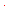
\includegraphics[width=3cm]{./GBToolPlotterDrawPoint.png}\\
\end{figure}
\end{center}

GBToolPlotterDrawPyramidoid.tga:\\
\begin{center}
\begin{figure}[H]
\centering
\includegraphics[width=3cm]{./GBToolPlotterDrawPyramidoid.png}\\
\end{figure}
\end{center}

testBottomLeft.tga:\\
\begin{center}
\begin{figure}[H]
\centering
\includegraphics[width=3cm]{./testBottomLeft.png}\\
\end{figure}
\end{center}

testTopLeft.tga:\\
\begin{center}
\begin{figure}[H]
\centering
\includegraphics[width=3cm]{./testTopLeft.png}\\
\end{figure}
\end{center}

GBSurfaceNormalizeHueTest.tga:\\
\begin{center}
\begin{figure}[H]
\centering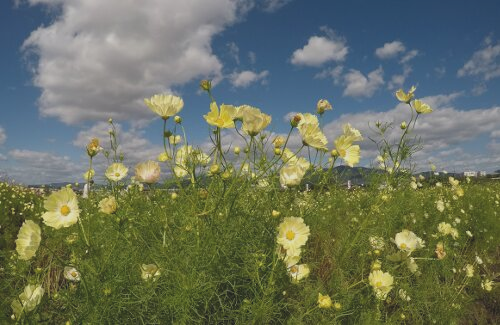
\includegraphics[width=6cm]{./GBSurfaceNormalizeHueTest.png}\\
\end{figure}
\end{center}

GBSurfaceNormalizeHueRef.tga:\\
\begin{center}
\begin{figure}[H]
\centering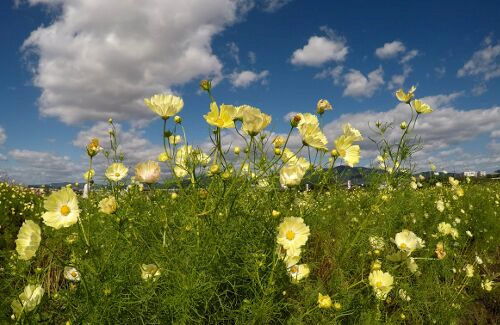
\includegraphics[width=6cm]{./GBSurfaceNormalizeHueRef.png}\\
\end{figure}
\end{center}

GBSurfaceOrderedDitheringTest.tga:\\
\begin{center}
\begin{figure}[H]
\centering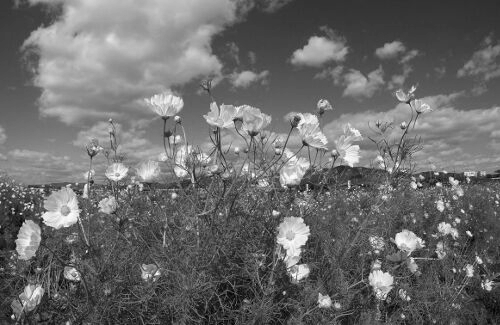
\includegraphics[width=6cm]{./GBSurfaceOrderedDitheringTest.png}\\
\end{figure}
\end{center}

GBSurfaceOrderedDitheringRef.tga:\\
\begin{center}
\begin{figure}[H]
\centering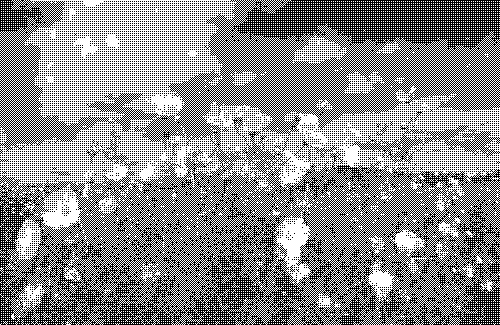
\includegraphics[width=6cm]{./GBSurfaceOrderedDitheringRef.png}\\
\end{figure}
\end{center}

GBSurfaceOrderedDitheringTestRGB.tga:\\
\begin{center}
\begin{figure}[H]
\centering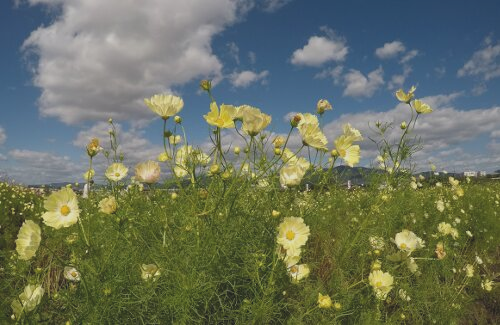
\includegraphics[width=6cm]{./GBSurfaceOrderedDitheringTestRGB.png}\\
\end{figure}
\end{center}

GBSurfaceOrderedDitheringRefRGB.tga:\\
\begin{center}
\begin{figure}[H]
\centering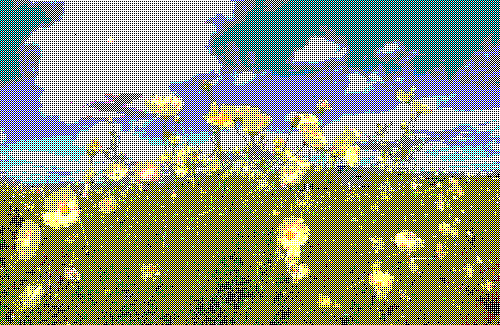
\includegraphics[width=6cm]{./GBSurfaceOrderedDitheringRefRGB.png}\\
\end{figure}
\end{center}

GBSurfaceFloydSteinbergDitheringTest.tga:\\
\begin{center}
\begin{figure}[H]
\centering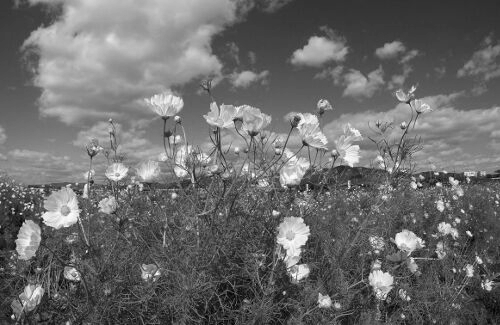
\includegraphics[width=6cm]{./GBSurfaceFloydSteinbergDitheringTest.png}\\
\end{figure}
\end{center}

GBSurfaceFloydSteinbergDitheringRef.tga:\\
\begin{center}
\begin{figure}[H]
\centering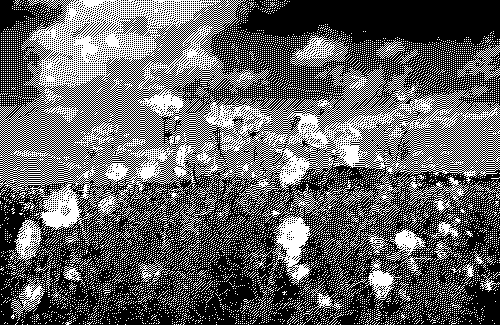
\includegraphics[width=6cm]{./GBSurfaceFloydSteinbergDitheringRef.png}\\
\end{figure}
\end{center}

GBSurfaceFloydSteinbergDitheringTestRGB.tga:\\
\begin{center}
\begin{figure}[H]
\centering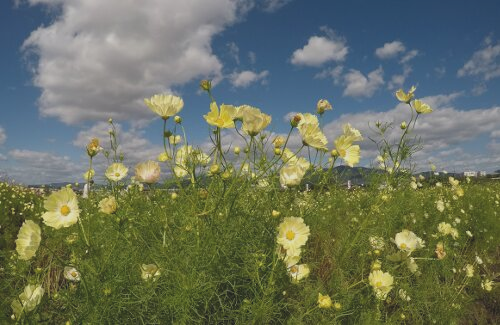
\includegraphics[width=6cm]{./GBSurfaceFloydSteinbergDitheringTestRGB.png}\\
\end{figure}
\end{center}

GBSurfaceFloydSteinbergDitheringRefRGB.tga:\\
\begin{center}
\begin{figure}[H]
\centering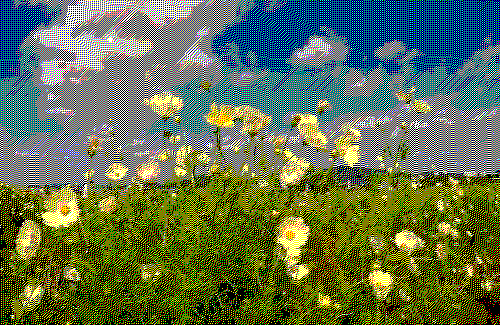
\includegraphics[width=6cm]{./GBSurfaceFloydSteinbergDitheringRefRGB.png}\\
\end{figure}
\end{center}

GBScaleCropTest.tga:\\
\begin{center}
\begin{figure}[H]
\centering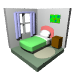
\includegraphics[width=6cm]{./GBScaleCropTest.png}\\
\end{figure}
\end{center}

GBScaleTestAvgNeighbourRef.tga:\\
\begin{center}
\begin{figure}[H]
\centering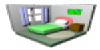
\includegraphics[width=6cm]{./GBScaleTestAvgNeighbourRef01.png}\\
\end{figure}
\end{center}

GBCropTestRef01.tga:\\
\begin{center}
\begin{figure}[H]
\centering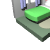
\includegraphics[width=6cm]{./GBCropTestRef01.png}\\
\end{figure}
\end{center}

GBCropTestRef02.tga:\\
\begin{center}
\begin{figure}[H]
\centering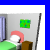
\includegraphics[width=6cm]{./GBCropTestRef02.png}\\
\end{figure}
\end{center}

screenshotGBSurfaceApp.tga:\\
\begin{center}
\begin{figure}[H]
\centering
\includegraphics[width=6cm]{./screenshotGBSurfaceApp.png}\\
\end{figure}
\end{center}

screenshotGBSurfaceWidget.tga:\\
\begin{center}
\begin{figure}[H]
\centering
\includegraphics[width=6cm]{./screenshotGBSurfaceWidget.png}\\
\end{figure}
\end{center}

\section{Demo}

\subsection{ImageViewer}

\subsubsection{main.c}

\begin{scriptsize}
\begin{ttfamily}
\verbatiminput{/home/bayashi/GitHub/GenBrush/Demo/ImageViewer/main.c}
\end{ttfamily}
\end{scriptsize}

\subsubsection{Makefile}

\begin{scriptsize}
\begin{ttfamily}
\verbatiminput{/home/bayashi/GitHub/GenBrush/Demo/ImageViewer/Makefile}
\end{ttfamily}
\end{scriptsize}

\subsection{Glade}

This example shows how to use a GenBrush widget within a GUI designed using Glade.

\subsubsection{main.c}

\begin{scriptsize}
\begin{ttfamily}
\verbatiminput{/home/bayashi/GitHub/GenBrush/Demo/Glade/main.c}
\end{ttfamily}
\end{scriptsize}

\subsubsection{Makefile}

\begin{scriptsize}
\begin{ttfamily}
\verbatiminput{/home/bayashi/GitHub/GenBrush/Demo/Glade/Makefile}
\end{ttfamily}
\end{scriptsize}

\subsubsection{test.glade}

\begin{scriptsize}
\begin{ttfamily}
\verbatiminput{/home/bayashi/GitHub/GenBrush/Demo/Glade/test.glade}
\end{ttfamily}
\end{scriptsize}
